\documentclass[10pt]{article} % use larger type; default would be 10pt

\usepackage[utf8]{inputenc} % set input encoding (not needed with XeLaTeX)
\usepackage{geometry} % to change the page dimensions
\geometry{a4paper} % or letterpaper (US) or a5paper or....
\usepackage{graphicx} % support the \includegraphics command and options
\usepackage{booktabs} % for much better looking tables
\usepackage{array} % for better arrays (eg matrices) in maths
\usepackage{paralist} % very flexible & customisable lists (eg. enumerate/itemize, etc.)
\usepackage{verbatim} % adds environment for commenting out blocks of text & for better verbatim
\usepackage{subfig} % make it possible to include more than one captioned figure/table in a single float
\usepackage{amsmath}
\usepackage{amssymb}
\usepackage{caption}
\usepackage{xcolor}
\usepackage{listings}
\usepackage{pgfplots}
\usepackage{tikz}
%\usepackage{float}
\usepackage{bm}
\usepackage[colorlinks,linkcolor=blue]{hyperref} % insert web link
\usepackage{multirow}

\usepackage{colortbl}
\usepackage{floatrow}
\floatsetup[table]
{capposition=top}
\newfloatcommand{capbtabbox}{table}
[][\FBwidth]

%% pseudocode
\usepackage{algorithm}
\usepackage{algorithmicx}
\usepackage{algpseudocode}
\usepackage{amssymb} %空集符号
\floatname{algorithm}{Discrete Logarithm Problem}
\renewcommand{\algorithmicrequire}{\textbf{Input:}}
\renewcommand{\algorithmicensure}{\textbf{Output:}}

\usepackage{mathtools}
\DeclarePairedDelimiter{\ceil}{\lceil}{\rceil}

\usepackage{color}
\definecolor{codegreen}{rgb}{0,0.6,0}
\definecolor{codegray}{rgb}{0.5,0.5,0.5}
\definecolor{codepurple}{rgb}{0.58,0,0.82}
\definecolor{backcolour}{rgb}{0.95,0.95,0.92}

\lstdefinestyle{mystyle}{
    backgroundcolor=\color{backcolour},
    commentstyle=\color{codegreen},
    keywordstyle=\color{magenta},
    numberstyle=\tiny\color{codegray},
    stringstyle=\color{codepurple},
    basicstyle=\footnotesize,
    breakatwhitespace=false,
    breaklines=true,
    captionpos=b,
    keepspaces=true,
    numbers=left,
    numbersep=5pt,
    showspaces=false,
    showstringspaces=false,
    showtabs=false,
    tabsize=2
}
\lstset{style=mystyle}

% These packages are all incorporated in the memoir class to one degree or another...
%%% HEADERS & FOOTERS
\usepackage{fancyhdr} % This should be set AFTER setting up the page geometry
\pagestyle{myheadings} % options: empty , plain , fancy
\markboth{left}{Report Template}
\renewcommand{\headrulewidth}{0pt} % customise the layout...
\lhead{}\chead{}\rhead{}
\lfoot{}\cfoot{\thepage}\rfoot{}
%%% SECTION TITLE APPEARANCE
\usepackage{sectsty}
\allsectionsfont{\sffamily\mdseries\upshape} % (See the fntguide.pdf for font help)
% (This matches ConTeXt defaults)
%%% ToC (table of contents) APPEARANCE
\usepackage[nottoc,notlof,notlot]{tocbibind} % Put the bibliography in the ToC
\usepackage[titles,subfigure]{tocloft} % Alter the style of the Table of Contents
\renewcommand{\cftsecfont}{\rmfamily\mdseries\upshape}
\renewcommand{\cftsecpagefont}{\rmfamily\mdseries\upshape} % No bold!
%%% END Article customizations
%%% The "real" document content comes below...
\setlength{\parindent}{0pt} % No indent

\title{Report}
\author{
{Zhang San}\\
\normalsize ID: 123456789\\
\normalsize Major: Electrical Engineering
}
\date{\today} % Activate to display a given date or no date (if empty),
         % otherwise the current date is printed

\begin{document}
\maketitle
%\tableofcontents

\begin{center}
\fbox{
\shortstack[l]{
Submission: Room $\#$301, Building No.1\\
Deadline: Jan. $1^{\text{st}}$, 2020}
}
\end{center}

\vspace{1cm}

\section{Text}
\textbf{Problem: This is a \LaTeX\;report template.}\\[10pt]

\subsection{Test}
%% insert single picture
\textbf{1. Insert pictures}
\begin{figure}[H] %h
  \centering
  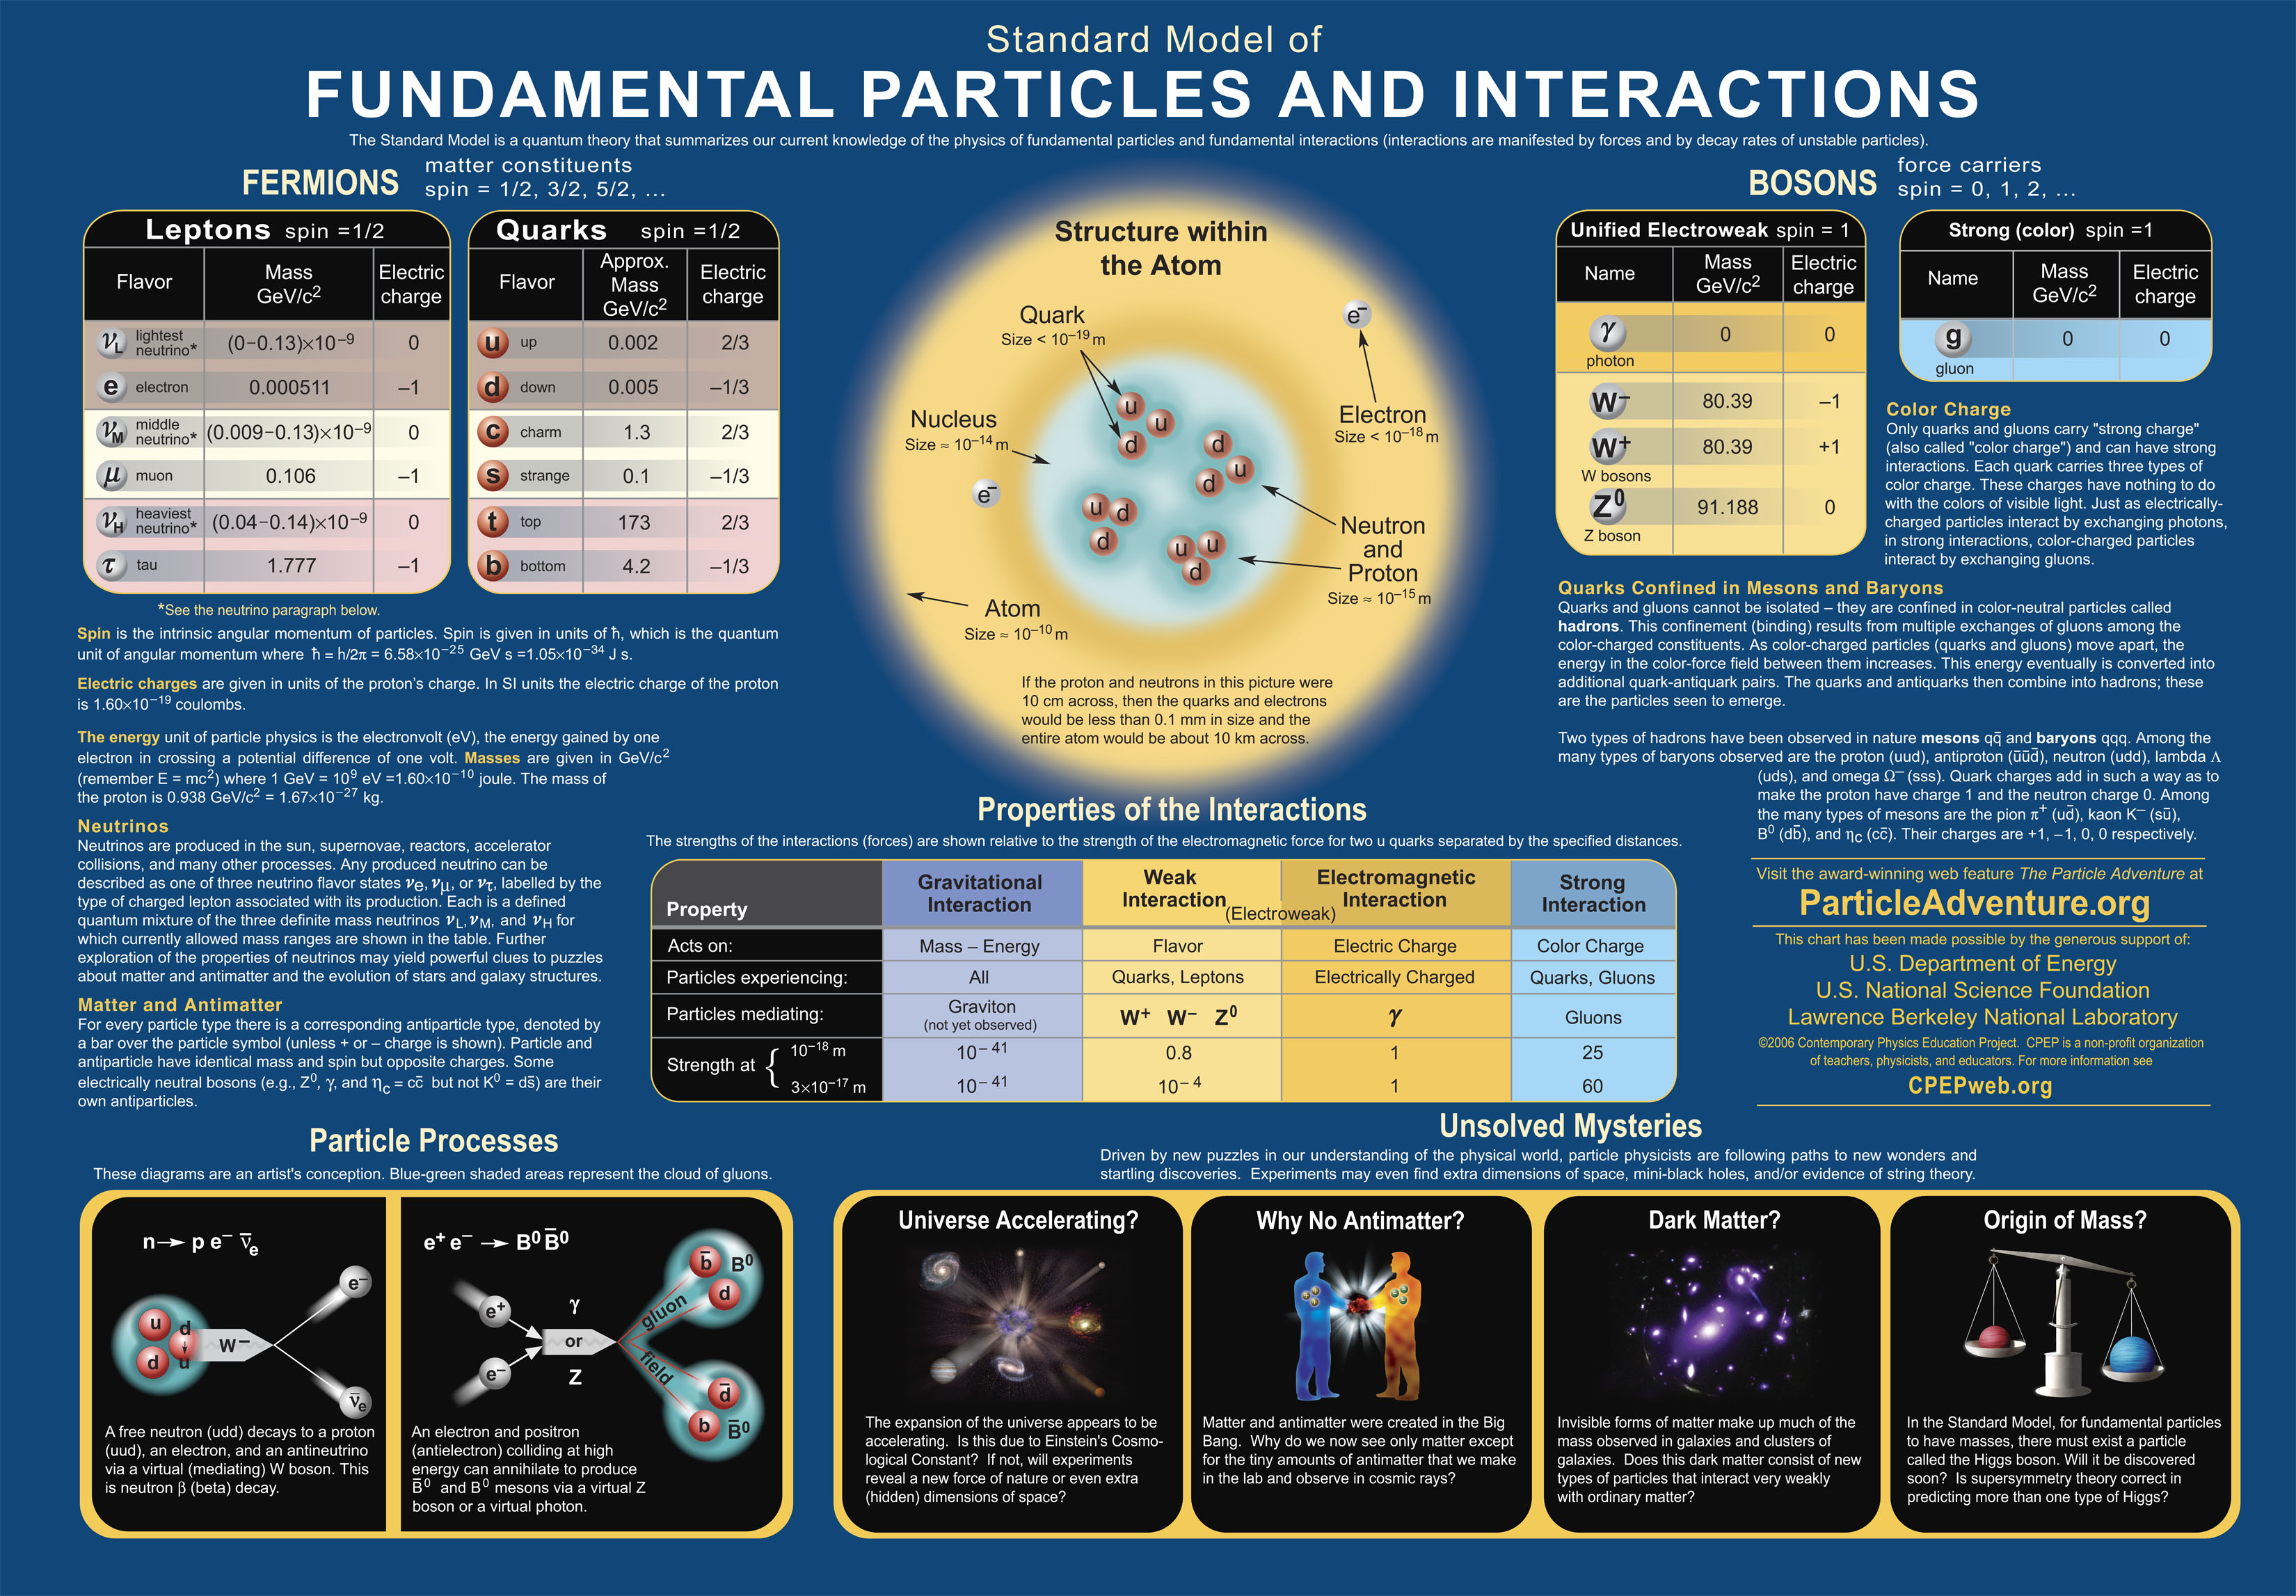
\includegraphics[width=0.5\textwidth]{eg1.jpg}
  \caption{example}\label{}
\end{figure}

%% insert multiple pictures
\begin{figure}[H] %h
  \centering
  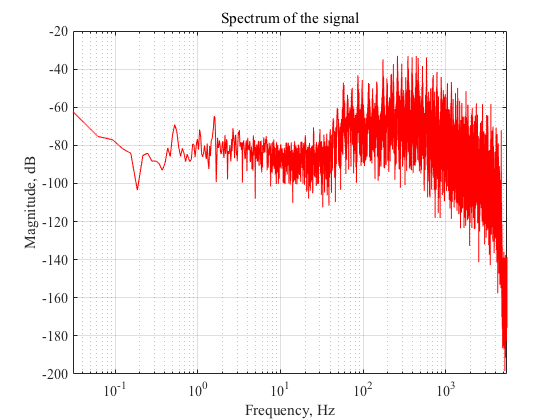
\includegraphics[width=0.4\textwidth]{m1.png}
  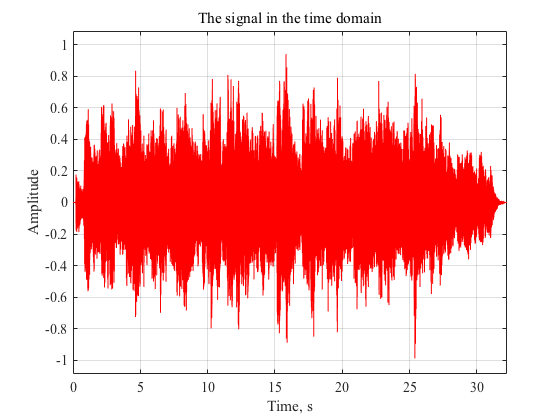
\includegraphics[width=0.4\textwidth]{m2.png}
  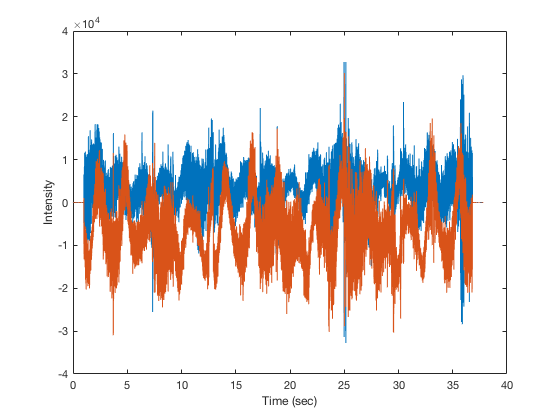
\includegraphics[width=0.4\textwidth]{m3.png}
  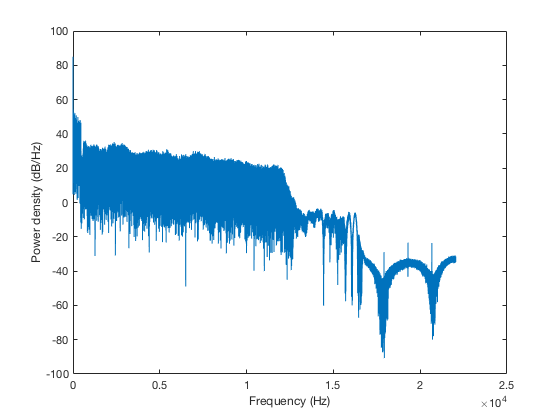
\includegraphics[width=0.4\textwidth]{m4.png}
  \caption{pictures}\label{}
\end{figure}

%% minipage
$\bullet$ Case 1:\\
\fbox{\begin{minipage}{14cm}
a\\
b\\
c\\
\end{minipage}
}\\[10pt]
Talk is cheap, show me the code.\\

%% 插入代码 colorbox
\textbf{2. insert code, colorbox}
\begin{colorboxed}
\begin{lstlisting}[language={[ANSI]R},numbers=left,numberstyle=\tiny,frame=shadowbox,
   rulesepcolor=\color{red!20!green!20!blue!20},
   keywordstyle=\color{blue!70!black},
   commentstyle=\color{blue!90!},
   basicstyle=\ttfamily]
> x <- c(26,29,27,25,29,27,26,29)
> y <- c(29,30,38,30,25,39,26,36)
\end{lstlisting}
\end{colorboxed}

%插入代码2
\textbf{3. insert code 2}
\begin{lstlisting}[language=Python, numbers=left, numberstyle=\tiny]
# -*- coding: utf-8 -*-

import math
import numpy as np
import matplotlib.pyplot as plt

def runga_kutta_vibrations(t, y0, v0, m, c, k):
    y = np.zeros(t.shape)
    v = np.zeros(t.shape)
    y[0] = y0
    v[0] = v0
    dt = t[1] - t[0]

    # Return the acceleration a
    def func(y, v):
        return (-c*v-k*y)/m
        
    for i in range(t.size - 1):
       # f_t_05 = (force[i+1] - force[i])/2 + force[i]
        y1 = y[i]
        v1 = v[i]
        a1 = func(y1, v1)
        y2 = y[i] + v1*dt/2
        v2 = v[i] + a1*dt/2
        a2 = func(y2, v2)
        y3 = y[i] + v2*dt/2
        v3 = v[i] + a2*dt/2
        a3 = func(y3, v3)
        y4 = y[i] + v3*dt
        v4 = v[i] + a3*dt
        a4 = func(y4, v4)
        y[i+1] = y[i] + dt*(v1 + 2*v2 + 2*v3 + v4)/6
        v[i+1] = v[i] + dt*(a1 + 2*a2 + 2*a3 + a4)/6

        print(y[i])
    return y

n = 400    ## set the grids
t = np.linspace(0, 4, n+1)   ## set time step
#force = np.zeros(n)   ## set the external force as zero

# Parameters of the vibration system
m = 1
k = 9*math.pi
omega = 3*math.pi
h = 0.2        # damping rate can be replaced as 1, 2, etc.
c = 2*m*h*omega
y = runga_kutta_vibrations(t, 3*math.sqrt(3), 0, m, c, k)

# Plot the result
plt.plot(t, y, 'r*', linewidth=1)
plt.xlabel('Time')
plt.ylabel('Amplitude')
plt.title('Damped free vibration h=0.2 (4thRunge-Kutta)')

#fig, ax1 = plt.subplots()
#l1 = ax1.plot(t, v, color='b', label="displacement")
#ax2 = ax1.twinx()
#l2=ax2.plot(t, force, color='r', label="force")

#lines = l1 + l2
#plt.legend(lines, [l.get_label() for l in lines])
#plt.show()
\end{lstlisting}

%% 伪代码
The pseudocode is as follows:\\
\begin{algorithm}[H]
    \caption{Baby-step Giant-step}
    \begin{algorithmic}[1] %显示行号,1是每行都显示
        \Require $y$, $g$, $p$, let $x = q\cdot m + r$, and hence seek $q$, $r$
        \Ensure $x$
        \State Define $m$ as $\ceil{\sqrt{p-1}}$
        \State Loops
        \For {x=0 to m}
        \If {$q$ is good for guess}
        \State Output $y=g^{qm+r}$
        \EndIf
        \EndFor
        \State Loops
        \For {$q$ in $m$}
        \State Compute $y\times g^{-qm}$
        \If {$g^r = g^{-qm}$}
        \State Output $x = qm+r$
        \Else { Go to find next value of $q$}
        \EndIf
        \EndFor
        \State Print all the possible solutions
        %\EndFunction
    \end{algorithmic}
\end{algorithm}

%% 表格
\textbf{4. Make tables}
\begin{table}[H]
\centering
\begin{tabular}{|c|c|c|c|c|c|c|c|c|}
\hline Product x & 26 & 29 & 27 & 25 & 29 & 27 & 26 & 29\\
\hline Product y & 29 & 30 & 38 & 30 & 25 & 39 & 26 & 36\\
\hline
\end{tabular}
\end{table}

\begin{table}[h]
\centering
\caption{Travel trips by bus}
\begin{tabular}{c|ccc|c}
 \hline       & Zone1 & Zone2 & Zone3 & Total\\
 \hline Zone1 & 200   & 500   & 800   & 1500\\
        Zone2 & 300   & 200   & 700   & 1200\\
        Zone3 & 600   & 700   & 300   & 1600\\
  \hline      & 1100  & 1400  & 1800  & 4300\\
  \hline
\end{tabular}
\end{table}

\begin{table}[h]
\begin{floatrow}
\capbtabbox{
 \begin{tabular}{|c|c|c|c|}
 \hline       & Zone1 & Zone2 & Zone3\\
 \hline Zone1 & 0.02 & 0.05 & 0.08\\
 \hline Zone2 & 0.03 & 0.02 & 0.07\\
 \hline Zone3 & 0.06 & 0.07 & 0.03\\
 \hline
 \end{tabular}
}{
  \caption{Bus share $S_{ij}(bus)$}
  \label{tab:tb1}
  }
\capbtabbox{
 \begin{tabular}{|c|c|c|c|}
 \hline       & Zone1 & Zone2 & Zone3\\
 \hline Zone1 & 0.11 & 0.07 & 0.02\\
 \hline Zone2 & 0.06 & 0.11 & 0.02\\
 \hline Zone3 & 0.02 & 0.07 & 0.09\\
 \hline
  \end{tabular}
}{
  \caption{Car share $S_{ij}(car)$}
  \label{tab:tb2}

  }
\end{floatrow}
\end{table}


\begin{table}[h]
\centering
\caption{Solution with Step Size h=0.01}
\scalebox{0.6}{
\begin{tabular}{|c|c|c|c|c|c|}
 \hline    x   & True Solution & Euler method & Heun method & Modified Euler method & 4th order Runge-Kutta method\\
 \hline 0.000  & 0.0000000 & 0.0000000 & 0.0000000  & 0.0000000  & 0.0000000\\
 \hline 0.010  & 0.0199000 & 0.0200000 & 0.0198995  & 0.0198998  & 0.0199000\\
 \hline 0.020  & 0.0396000 & 0.0397990 & 0.0395990  & 0.0395995  & 0.0396000\\
 \hline 0.030  & 0.0591000 & 0.0593970 & 0.0590985  & 0.0590993  & 0.0591000\\
 \hline 0.040  & 0.0784000 & 0.0787940 & 0.0783980  & 0.0783990  & 0.0784000\\
 \hline 0.050  & 0.0975000 & 0.0979901 & 0.0974976  & 0.0974988  & 0.0975000\\
 \hline \vdots & \vdots & \vdots & \vdots & \vdots & \vdots\\
 \hline 0.960  & 1.0098187 & 1.0157715 & 1.0097903  & 1.0098030  & 1.0098187\\
 \hline 0.970  & 1.0111022 & 1.0170842 & 1.0110738  & 1.0110865  & 1.0111022\\
 \hline 0.980  & 1.0122088 & 1.0182193 & 1.0121803  & 1.0121930  & 1.0122088\\
 \hline 0.990  & 1.0131391 & 1.0191776 & 1.0131105  & 1.0131232  & 1.0131391\\
 \hline 1.000  & 1.0138938 & 1.0199596 & 1.0138651  & 1.0138778  & 1.0138938\\
 \hline
\end{tabular}}
\end{table}


\begin{table}
\centering
\caption{Comparison of accuracy}
\scalebox{0.6}{
  \begin{tabular}{|c|c|c|c|c|c|c|c|c|}
    \hline
    \multirow{2}{*}{Step Size} &
      \multicolumn{2}{c|}{Euler} &
      \multicolumn{2}{c|}{Heun} &
      \multicolumn{2}{c|}{Modified Euler} &
      \multicolumn{2}{c|}{4th Runge-Kutta} \\
        & Approximation & Error & Approximation & Error & Approximation & Error &  Approximation & Error\\
\hline 0.2 & 1.1431393 & 0.1292454 & 1.0011505 & 0.0127434&1.0067767&0.0071172&1.0138742&0.0000197\\
\hline 0.1 & 1.0763404 & 0.0624465 & 1.0108764 & 0.0030175&1.0122102&0.0016837&1.0138927&0.0000012\\
\hline 0.01& 1.0199596 & 0.0060658 & 1.0138651 & 0.0000287&1.0138778&0.0000161&1.0138938&0.0000000\\
\hline
  \end{tabular}}
\end{table}

\begin{table}[H]
\begin{tabular}{|c|c|c|c|c|c|c|c|c|c|c|}
\hline
\rowcolor[gray]{0.0}
\textcolor{white}{Last digit}&\textcolor{white}{0}&\textcolor{white}{1}&\textcolor{red}{2}&\textcolor{white}{3}&\textcolor{white}{4}&\textcolor{white}{5}
&\textcolor{white}{6}&\textcolor{white}{7}&\textcolor{white}{8}&\textcolor{white}{9}\\
\rowcolor[gray]{0.8}
ubackward&1.0&1.25&\textcolor{red}{1.5}&1.75&2.0&2.25&2.5&2.75&3.0&3.25\\
\hline
\end{tabular}
\end{table}


%% 矩阵、数学公式
\textbf{5. Equations}
$$
W = \frac{b^2}{S^2} = \frac{(\Sigma_{i=1}^{n}a_i x_{(i)})^2}{\Sigma_{i=1}^n(x_i - \bar{x})^2}
$$

$$
\Phi^{\ast} = \frac{(\frac{V_x}{n_x} + \frac{V_y}{n_y})^2}{(\frac{V_x}{n_x})^2\frac{1}{n_x -1} + (\frac{V_y}{n_y})^2\frac{1}{n_y -1}}
$$

$$\mathbf{B}=
\left(
\begin{array}{ccc}
\frac{\partial}{\partial x} & 0 \\
0 & \frac{\partial}{\partial y} \\
\frac{\partial}{\partial y} & \frac{\partial}{\partial x} \\
\end{array}
\right)
$$


$$
[\mathbf{C}]= \frac{E}{1-\nu^2}
\left(
\begin{array}{ccc}
1 & \nu & 0 \\
\nu & 1 & 0 \\
0 & 0 & \frac{1-\nu}{2} \\
\end{array}
\right)
$$

\begin{equation}
X = \begin{bmatrix}
1 & x_{11} & x_{21} & \ldots & x_{m1}\\
1 & x_{12} & x_{22} & \ldots & x_{m2}\\
\vdots & \vdots & \vdots & \ddots & \vdots\\
1 & x_{1n} & x_{2n} & \ldots & x_{mn}\\
\end{bmatrix},
Y = \begin{bmatrix}
y_0\\
y_1\\
\vdots\\
y_n
\end{bmatrix}
\end{equation}

\begin{equation}
\begin{split}
S_W = &\sum\limits_{k=1,2}\sum\limits_{x\in w_i} (w^Tx-w^T\mu_i)(w^Tx-w^T\mu_i)^T\\
= &\sum\limits_{x\in w_1}(w^Tx-w^T\mu_i)^2 + \sum\limits_{x\in w_2}(w^Tx-w^T\mu_i)^2\\
= &w^T(\tilde{s}_1+\tilde{s}_2)w\\
= &w^TS_Ww
\end{split}
\end{equation}

For free electrons, $E(k) = \frac{\hbar^2 k^2}{2m}$, and in the k space, the radius k for equal energy surface is $k = \sqrt{2mE}/\hbar$, volume V is $(2\pi/L)^3$\\
$$
|\nabla_k E| = \frac{dE}{dk} = \hbar^2k/m
$$
\begin{equation*}
\begin{split}
Z(E) &= \frac{L^3}{4\pi^3}\iint_{E=const}\frac{dS}{|\nabla_kE(k)|} = \frac{L^3}{4\pi^3}\iint_E dS\\
     &= \frac{L^3}{4\pi^3}\cdot\frac{m}{\hbar^2 k}\cdot 4\pi k^2 = \frac{(2m)^{3/2}L^3}{2\pi^2\hbar^3}E^{1/2} = 8\pi\sqrt{2}\frac{m^{3/2}}{(2\pi\hbar)^3}E^{1/2}\cdot L^3
\end{split}
\end{equation*}

(a) Prediction step in the y direction:\\

$$
{v^{p}_{i,j}=
\underbrace{v_{i,j}^{n}}_\text{v$\_$center}
+ \Delta t[-
\begingroup
\color{red}
\overbrace{\color{black}u^{n}_{i,j}\frac{\partial v_{i,j}^{n}}{\partial x}}^\text{\color{black}advection$\_$x}
\endgroup
-
\begingroup
\color{red}
\overbrace{\color{black}v_{i,j}^{n}\frac{\partial v_{i,j}^n}{\partial y}}^\text{\color{black}advection$\_$y}
\endgroup
- \underbrace{\frac{1}{\rho}\frac{\partial p_{i,j}^n}{\partial y}}_\text{pressure$\_$y} +
\begingroup
\color{blue}
\overbrace{\color{black}\nu\frac{\partial^2 u_{i,j}^n}{\partial x^2}}^\text{\color{black}diffusion$\_$x}
\endgroup
+
\begingroup
\color{blue}
\overbrace{\color{black}\nu\frac{\partial^2 v_{i,j}^n}{\partial y^2}}^\text{\color{black}diffusion$\_$y}
\endgroup
]}
$$

(b) Advection term:\\
Using first-order upwind difference scheme:\\
\begin{equation*}
c\frac{\partial f_i}{\partial x}|^n =
\left\{
             \begin{array}{c}
                c\dfrac{f_i^n- f_{i-1}^n}{\Delta x}, \text{c}\geq 0 \Rightarrow c*(\text{f}_\text{center} - \text{f}_\text{minus})/\text{delta}\\
                \vspace{5mm}
                c\dfrac{f_{i+1}^n- f_{i}^n}{\Delta x},  c<0 \Rightarrow \text{c}*(\text{f}_\text{plus} -\text{f}_\text{center})/\text{delta}
             \end{array}
\right
\end{equation*}

\textbf{6. Let your student ID be "A" and the remainder of dividing "A" by 6 be "C". Compute "D=21+C", show an algorithm that computes a non-zero "E" where \bm{$E=exp(-(D-0.5)^2)*exp(-(D+0.5)^2)/exp(-D^2)$}.}\\[10pt]
web site \href{http://www-pw.physics.uiowa.edu/rbsp/audio/}{http://www-pw.physics.uiowa.edu/rbsp/audio/}.\\[10pt]
Integral:\\
$$
\int\limits_{V}\rho\frac{d\mathbf{v}}{dt}dV = \int\limits_{V}\mathbf{b}dV + \int\limits_{V}\mathbf{B}^T\mathbf{\sigma}dV
$$

$$
\mathbf{u}(x)=\sum\limits_{i=1}^{2} h_i u_i
$$

$$
\Phi(a_nx+b_n)^n = (\frac{1}{\sqrt{2\pi}}\int_{-\infty}^{a_nx+b_n} e^{-\frac{y^2}{2}}dy)^n \rightarrow e^{-e^{-x}}
$$

\vspace{1cm}

\textbf{References:}\\[5pt]
[1] S. M. Sze, Semiconductor Devices: Physics and Technology, 3rd edition.\\

[2] Stephen J. Chapman. Fortran 95/2003 for Scientists and Engineers, 3rd edition. McGraw-Hill Education. 2007.\\

[3] Gilbert Strang. An Analysis of the Finite Element Method, 2nd edition. Wellesley-Cambridge. 2008.\\

[4] Jochen Alberty, Carsten Carstensen, Stefan A. Funken. Remarks around 50 lines of Matlab: short finite element implementation. Numerical Algorithms 20(1999)117-137.


\end{document}
